\documentclass[10pt, a4paper]{article}

\usepackage{ctex}
\usepackage{xeCJK}
\usepackage{caption}
\usepackage{geometry}
\geometry{
    left = 0.6in,
    right = 0.6in,
    top = 0.8in,
    bottom = 1.0in
}
\usepackage{amssymb}
\usepackage{amsbsy}
\usepackage{amsmath}
\usepackage{xcolor}
\usepackage{mathrsfs}
\usepackage{graphicx}
\usepackage{tasks}
\settasks{
    label = \Alph*. ,
    label-width = 16pt
}
\pagestyle{empty}

\newcommand{\Title}[3]{
    \begin{center}
        \Large \textbf{中国电子学会 #1~年~#2~月 Scratch~#3级考试}
    \end{center}
}
\newcommand{\TimeAndName}[1]{
    \begin{center}
        考试时间:~#1~ 分钟 \qquad\qquad\qquad\qquad 姓名:\underline{\quad\quad\quad\quad}
    \end{center}
}

\begin{document}
    \Title{2022}{6}{一} % 标题
    \TimeAndName{60} % 考试时间及姓名

    % 单选题
    \vspace{2mm}
    {\noindent\textbf{第一部分、单选题(共 25 题,每题 2 分,共50分.)}}
    \begin{enumerate}
        % 1
        \item 广场中有声控喷泉,当声音的音量大于 60 的时候,喷泉就会喷出水,现在的音量为 30,下列哪个选项可以让喷泉喷出水?(\qquad)
        \begin{tasks}(4)
            \task 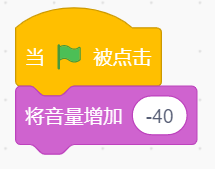
\includegraphics[width=.12\textwidth]{1a.png}
            \task 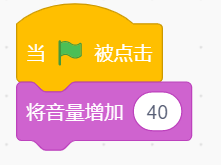
\includegraphics[width=.12\textwidth]{1b.png}
            \task 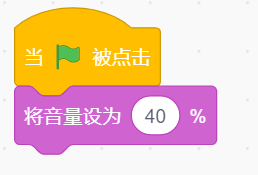
\includegraphics[width=.15\textwidth]{1c.png}
            \task 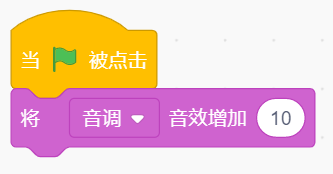
\includegraphics[width=.18\textwidth]{1d.png}
        \end{tasks}

        % 2
        \item 造型编辑器中,选中橙子以及它的阴影后,点击下面哪个按钮可以让造型从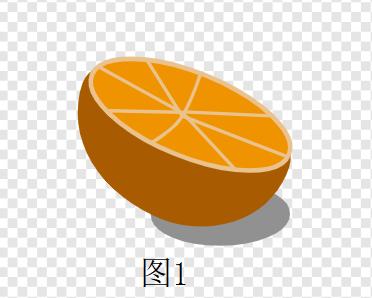
\includegraphics[width=.08\textwidth]{2-1.png}变成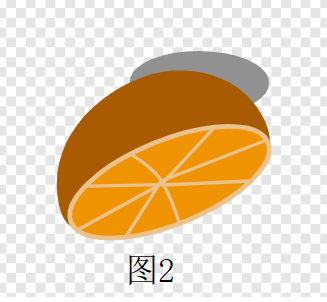
\includegraphics[width=.07\textwidth]{2-2.png}?(\qquad)
        \begin{tasks}(4)
            \task 
\includegraphics[width=.05\textwidth]{2a.png}
            \task 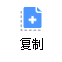
\includegraphics[width=.05\textwidth]{2b.png}
            \task 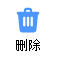
\includegraphics[width=.05\textwidth]{2c.png}
            \task 
\includegraphics[width=.05\textwidth]{2d.png}
        \end{tasks}

        % 3
        \item 小猫和小狗比赛,下图的黑线是终点,两个角色初始位置距离终点都是50步,点击绿旗后,谁先到达终点?(\qquad)
        \begin{tasks}(4)
            \task 小猫
            \task 小狗
            \task 同时到达
            \task 不一定
        \end{tasks}

        % 4
        \item 下面选项说法错误的是?(\qquad)
        \begin{tasks}
            \task 舞台区可以同时展示多个角色,但是只能同时展示一个背景
            \task 角色的造型有位图和矢量图两种模式
            \task 作品名称只能在编程界面修改,不能在保存到电脑时修改
            \task 不使用积木块也可以设置角色的旋转方式
        \end{tasks}

        % 2,4,6 图片
        \begin{figure}[htbp]
            \begin{minipage}[t]{.4\textwidth}
                \centering
                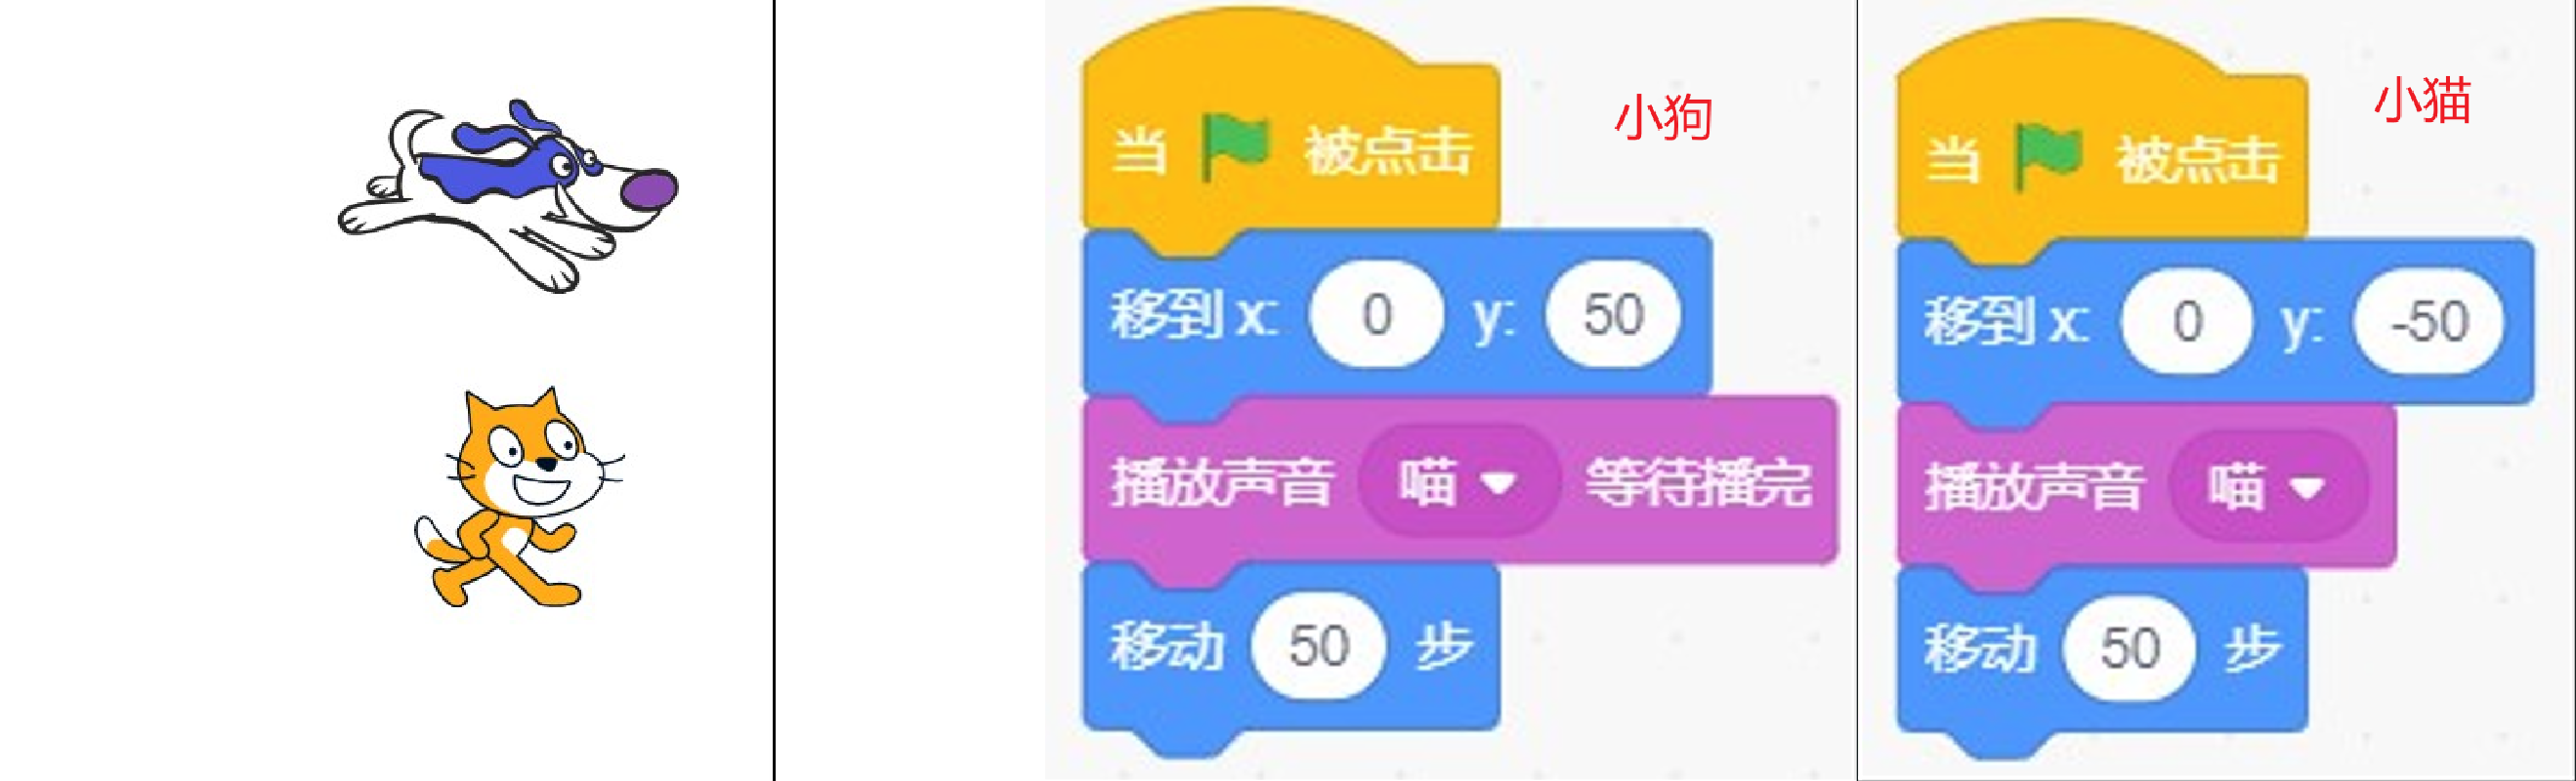
\includegraphics[width=\textwidth]{3.png}
                \caption*{第 3 题}
            \end{minipage}
            \begin{minipage}[t]{.3\textwidth}
                \centering
                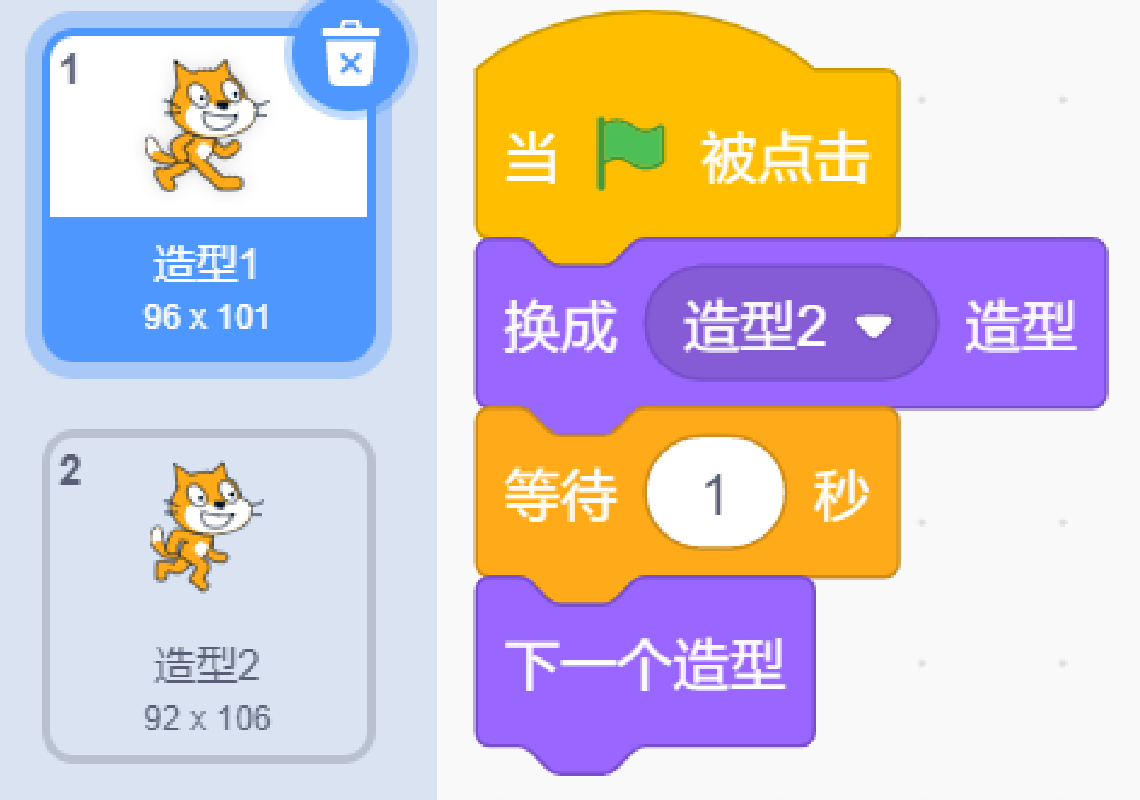
\includegraphics[width=.6\textwidth]{5.png}
                \caption*{第 5 题}
            \end{minipage}
            \begin{minipage}[t]{.28\textwidth}
                \centering
                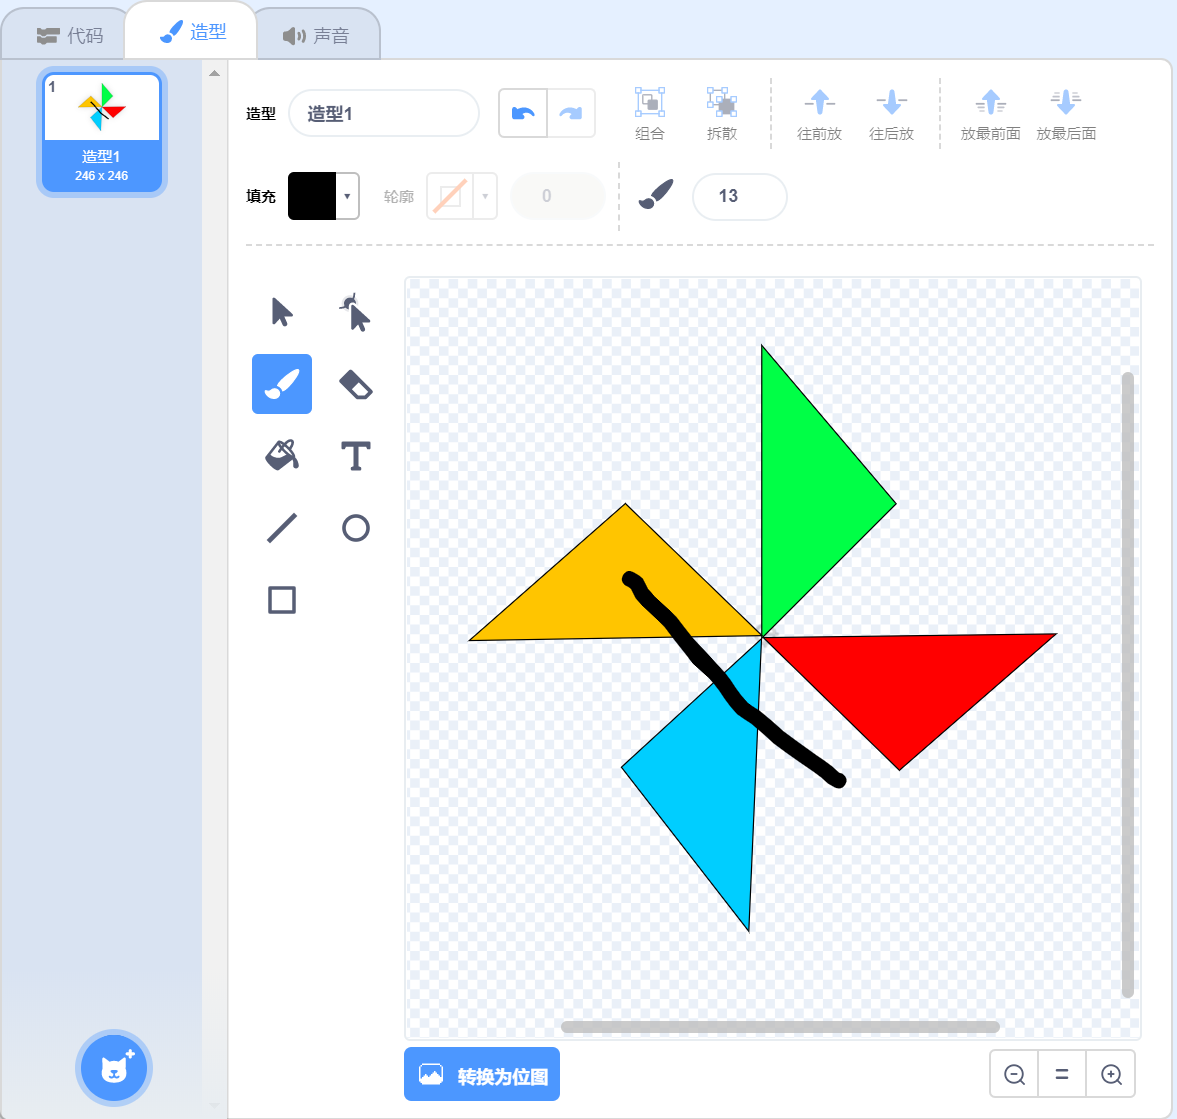
\includegraphics[width=.6\textwidth]{6.png}
                \caption*{第 6 题}
            \end{minipage}
        \end{figure}

        % 5
        \item 如上图所示,小猫有两个造型,程序执行结束后,小猫的造型是?(\qquad)
        \begin{tasks}(4)
            \task 造型1
            \task 造型2
            \task 都有可能
            \task 两个造型会不停切换
        \end{tasks}

        % 6
        \item 如上图所示,绘制完风车的图案后,不小心画错了,多画了一条黑色的线。下列哪个选项能够让风车立刻变回原来的样子?(\qquad)
        \begin{tasks}(4)
            \task 
\includegraphics[width=.04\textwidth]{6a.png}
            \task 
\includegraphics[width=.04\textwidth]{6b.png}
            \task 
\includegraphics[width=.04\textwidth]{6c.png}
            \task 
\includegraphics[width=.04\textwidth]{6d.png}
        \end{tasks}

        \newpage
        % 7
        \item Ben角色的造型列表如下图所示,下列选项中,造型名称和造型编号对应正确的是?(\qquad)
        \begin{tasks}(2)
            \task 造型名称ben-a对应造型编号0
            \task 造型名称ben-b对应造型编号2
            \task 造型名称ben-c对应造型编号1
            \task 造型名称ben-d对应造型编号3
        \end{tasks}

        % 8
        \item 舞台的两个背景如下图所示,小猫每天先去篮球场打球3分钟,再去游泳池游泳。下面哪个选项能正确表示运动场景变化?(\qquad)
        \begin{tasks}(4)
            \task 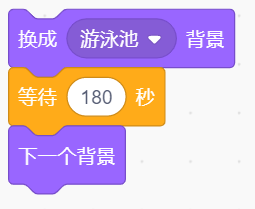
\includegraphics[width=.14\textwidth]{8a.png}
            \task 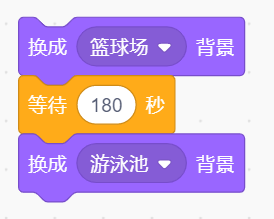
\includegraphics[width=.14\textwidth]{8b.png}
            \task 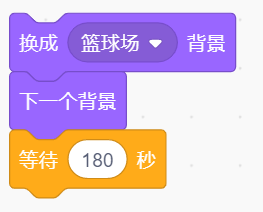
\includegraphics[width=.14\textwidth]{8c.png}
            \task 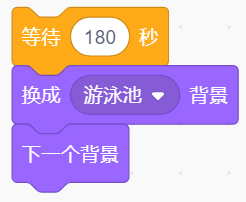
\includegraphics[width=.14\textwidth]{8d.png}
        \end{tasks}

         % 8,10,11,12 图片
         \begin{figure}[htbp]
            \centering
            \begin{minipage}[t]{.08\textwidth}
                \centering
                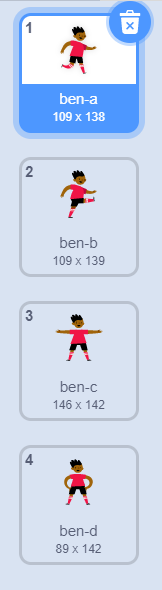
\includegraphics[width=\textwidth]{7.png}
                \caption*{第 7 题}
            \end{minipage}
            \begin{minipage}[t]{.12\textwidth}
                \centering
                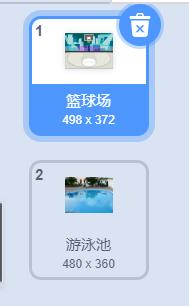
\includegraphics[width=\textwidth]{8.png}
                \caption*{第 8 题}
            \end{minipage}
            \begin{minipage}[t]{.12\textwidth}
                \centering
                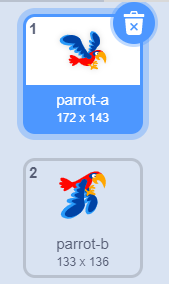
\includegraphics[width=\textwidth]{9.png}
                \caption*{第 9 题}
            \end{minipage}
            \begin{minipage}[t]{.3\textwidth}
                \centering
                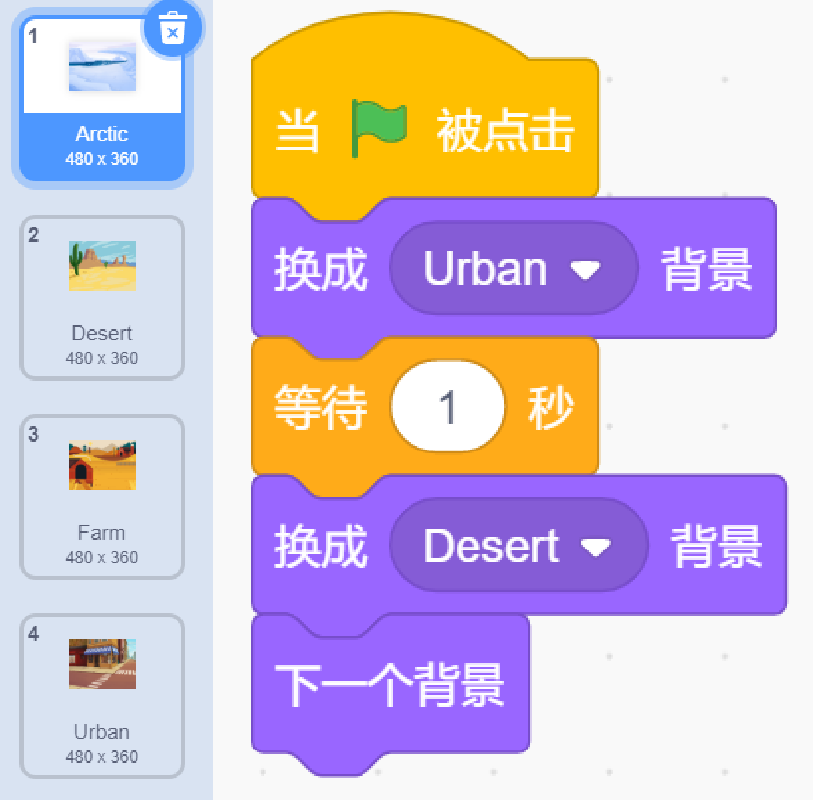
\includegraphics[width=\textwidth]{10.png}
                \caption*{第 10 题}
            \end{minipage}
            \begin{minipage}[t]{.33\textwidth}
                \centering
                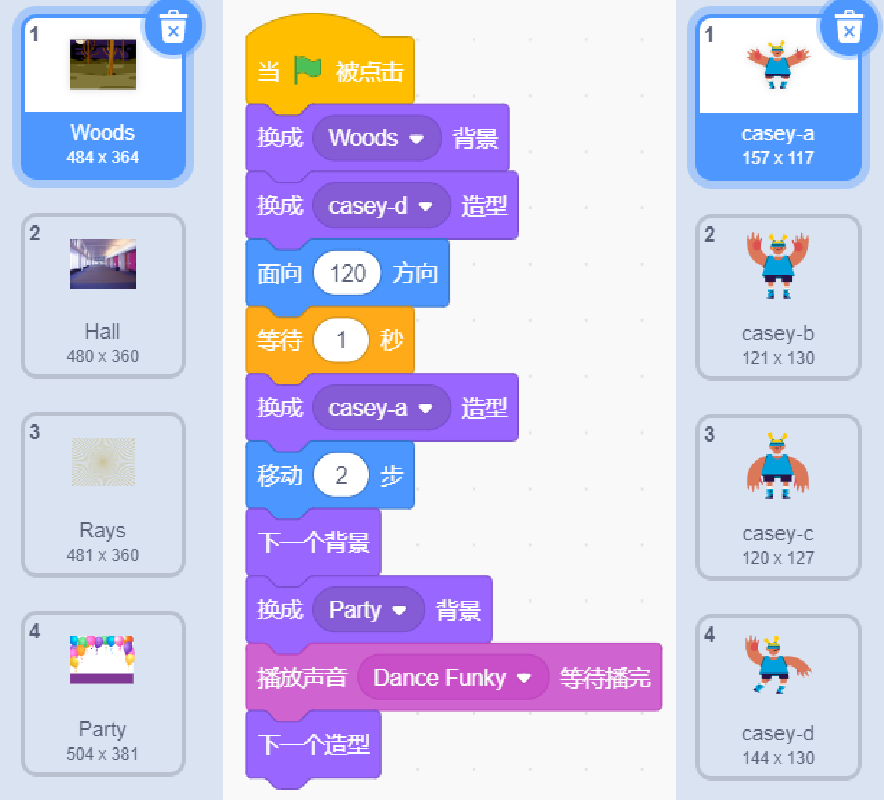
\includegraphics[width=\textwidth]{11.png}
                \caption*{第 11 题}
            \end{minipage}
        \end{figure}

        % 9
        \item Parrot有两个造型,下列选项程序执行结束后,能够看到Parrot多次挥舞翅膀效果的是?(\qquad)
        \begin{tasks}(4)
            \task 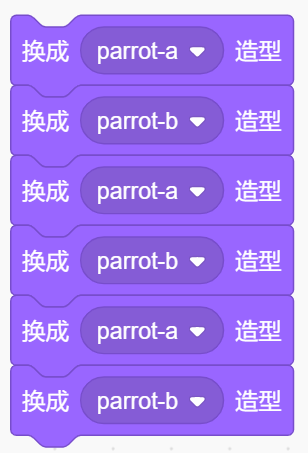
\includegraphics[width=.13\textwidth]{9a.png}
            \task 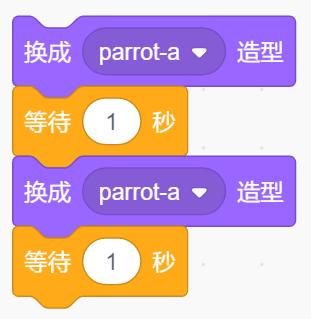
\includegraphics[width=.15\textwidth]{9b.png}
            \task 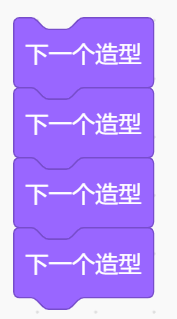
\includegraphics[width=.11\textwidth]{9c.png}
            \task 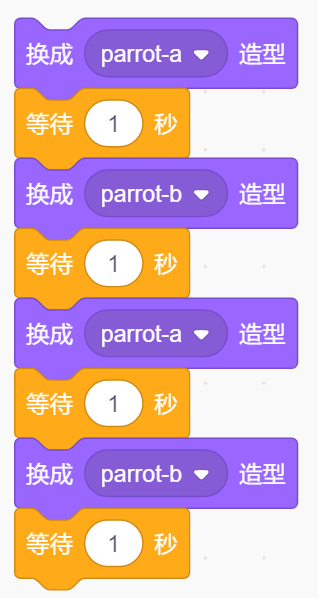
\includegraphics[width=.11\textwidth]{9d.png}
        \end{tasks}

        % 10
        \item 舞台有如下背景,程序执行结束后,舞台最终显示的背景是?(\qquad)
        \begin{tasks}(4)
            \task Arctic
            \task Desert
            \task Farm
            \task Urban
        \end{tasks}

        % 11
        \item Casey的造型列表和舞台的背景列表如上图所示。当程序执行结束后,正确显示舞台区的背景和角色造型的是哪一个选项?(\qquad)
        \begin{tasks}(4)
            \task 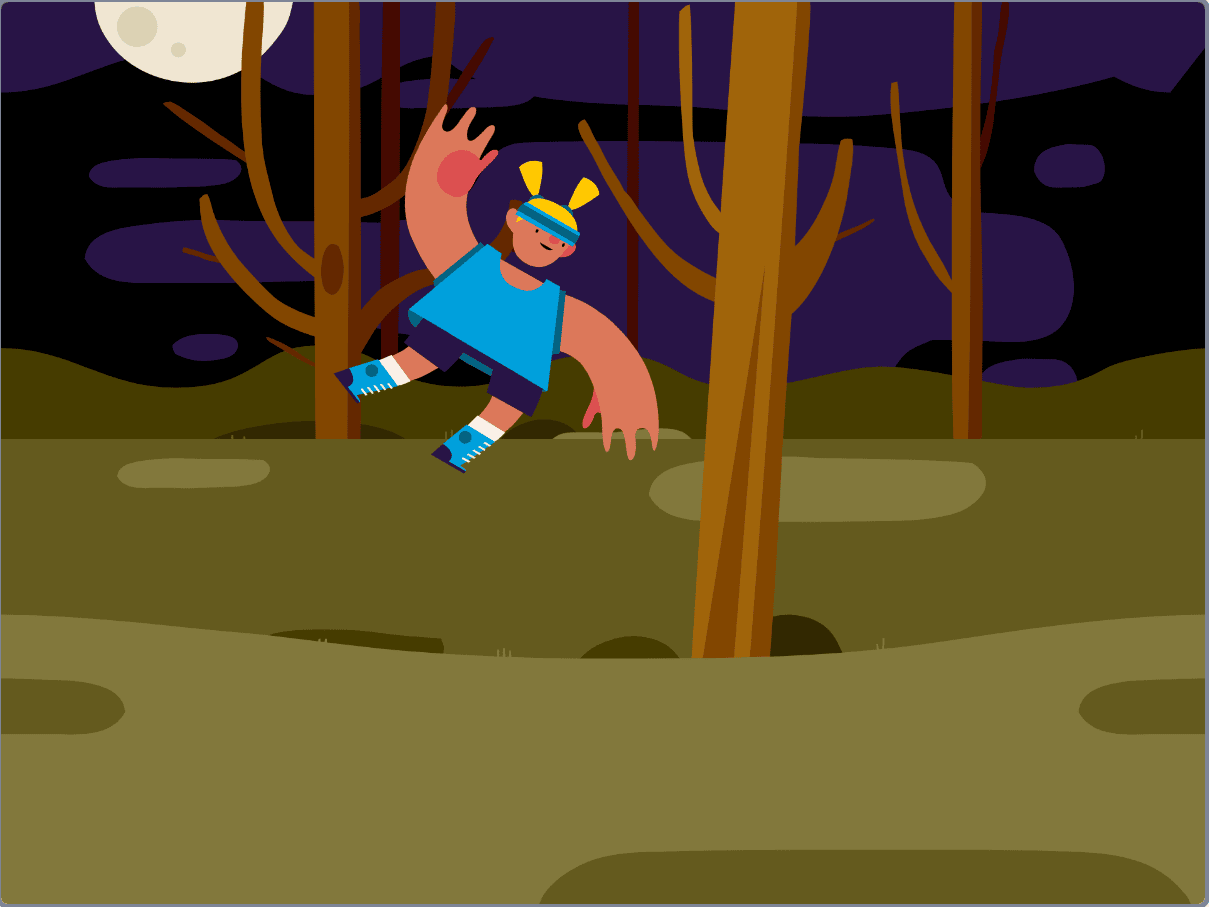
\includegraphics[width=.15\textwidth]{11a.png}
            \task 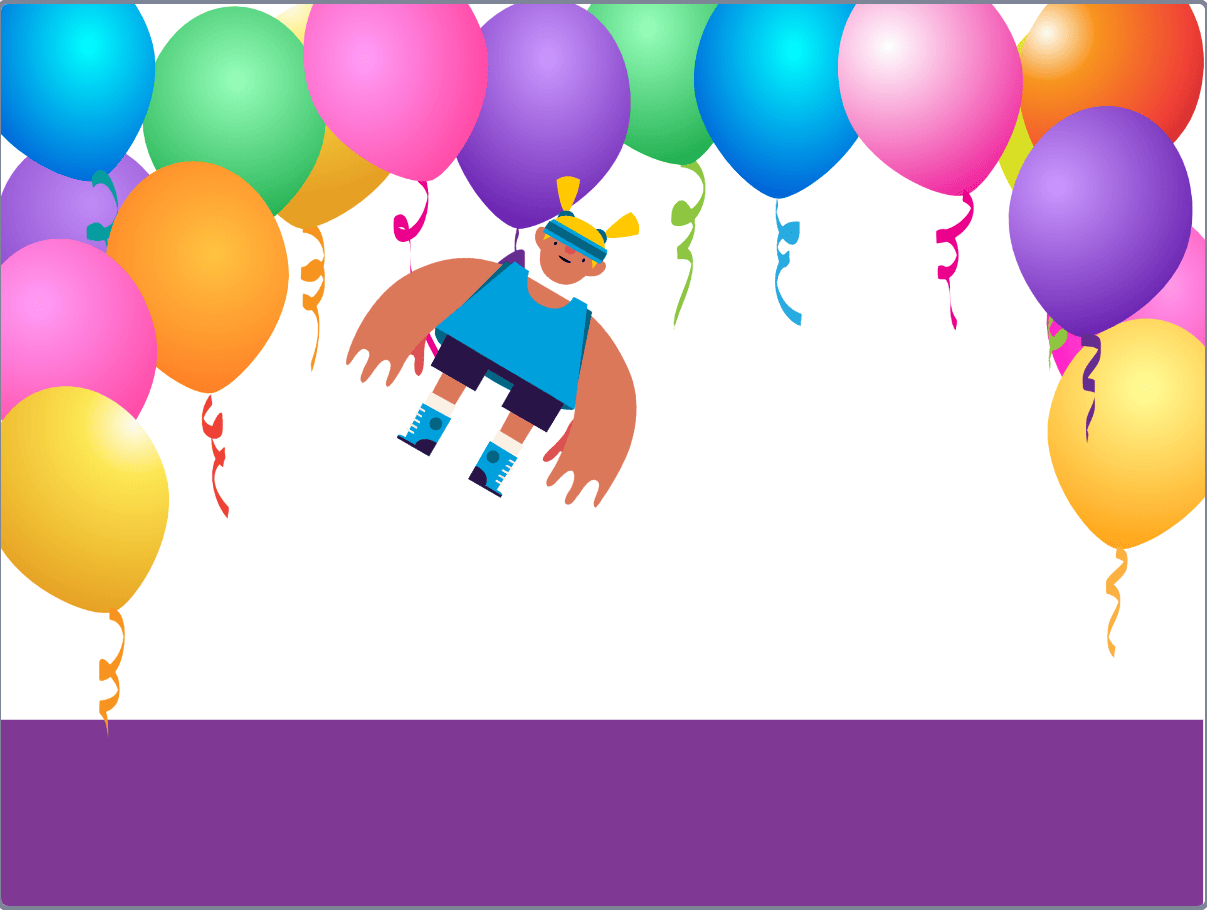
\includegraphics[width=.15\textwidth]{11b.png}
            \task 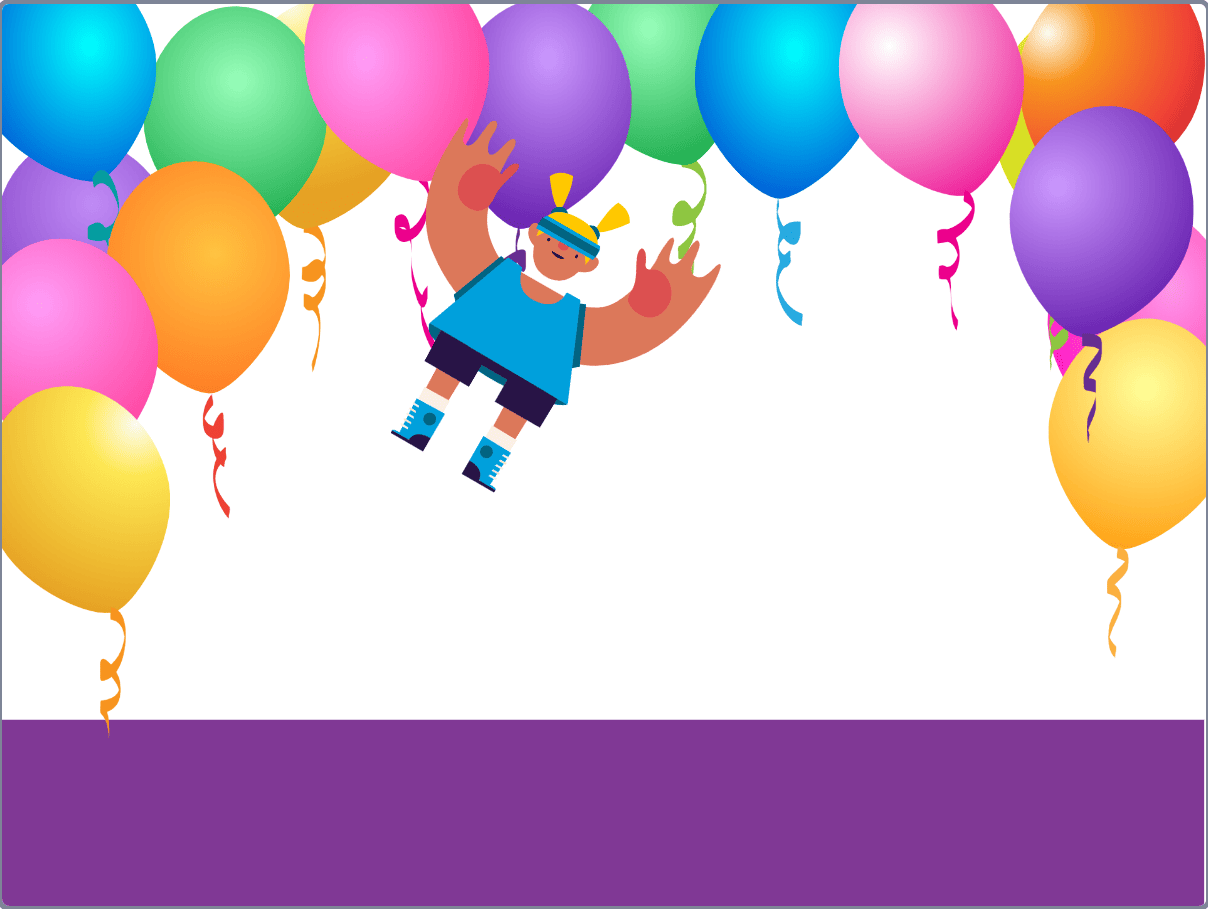
\includegraphics[width=.15\textwidth]{11c.png}
            \task 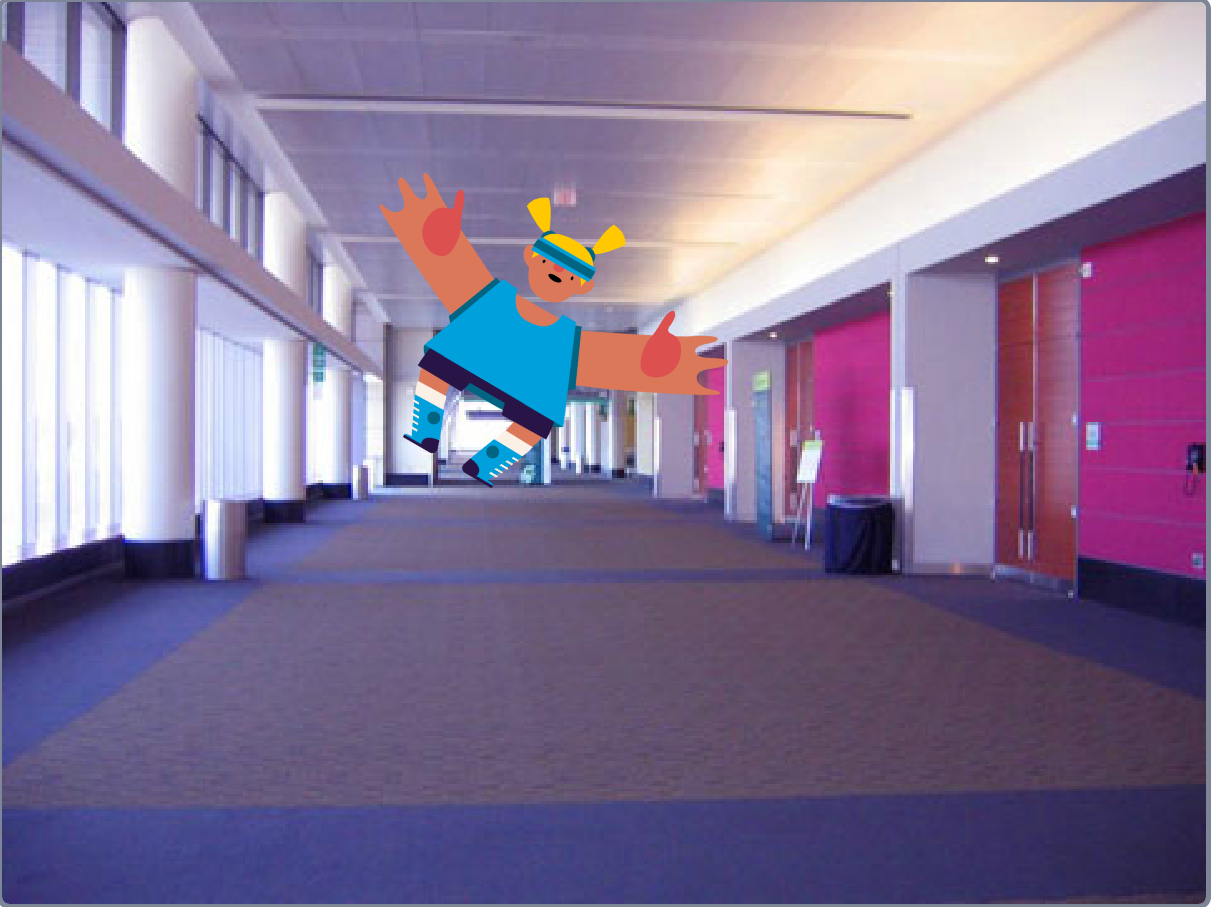
\includegraphics[width=.15\textwidth]{11d.png}
        \end{tasks}

        % 12
        \item 两根木棒,如图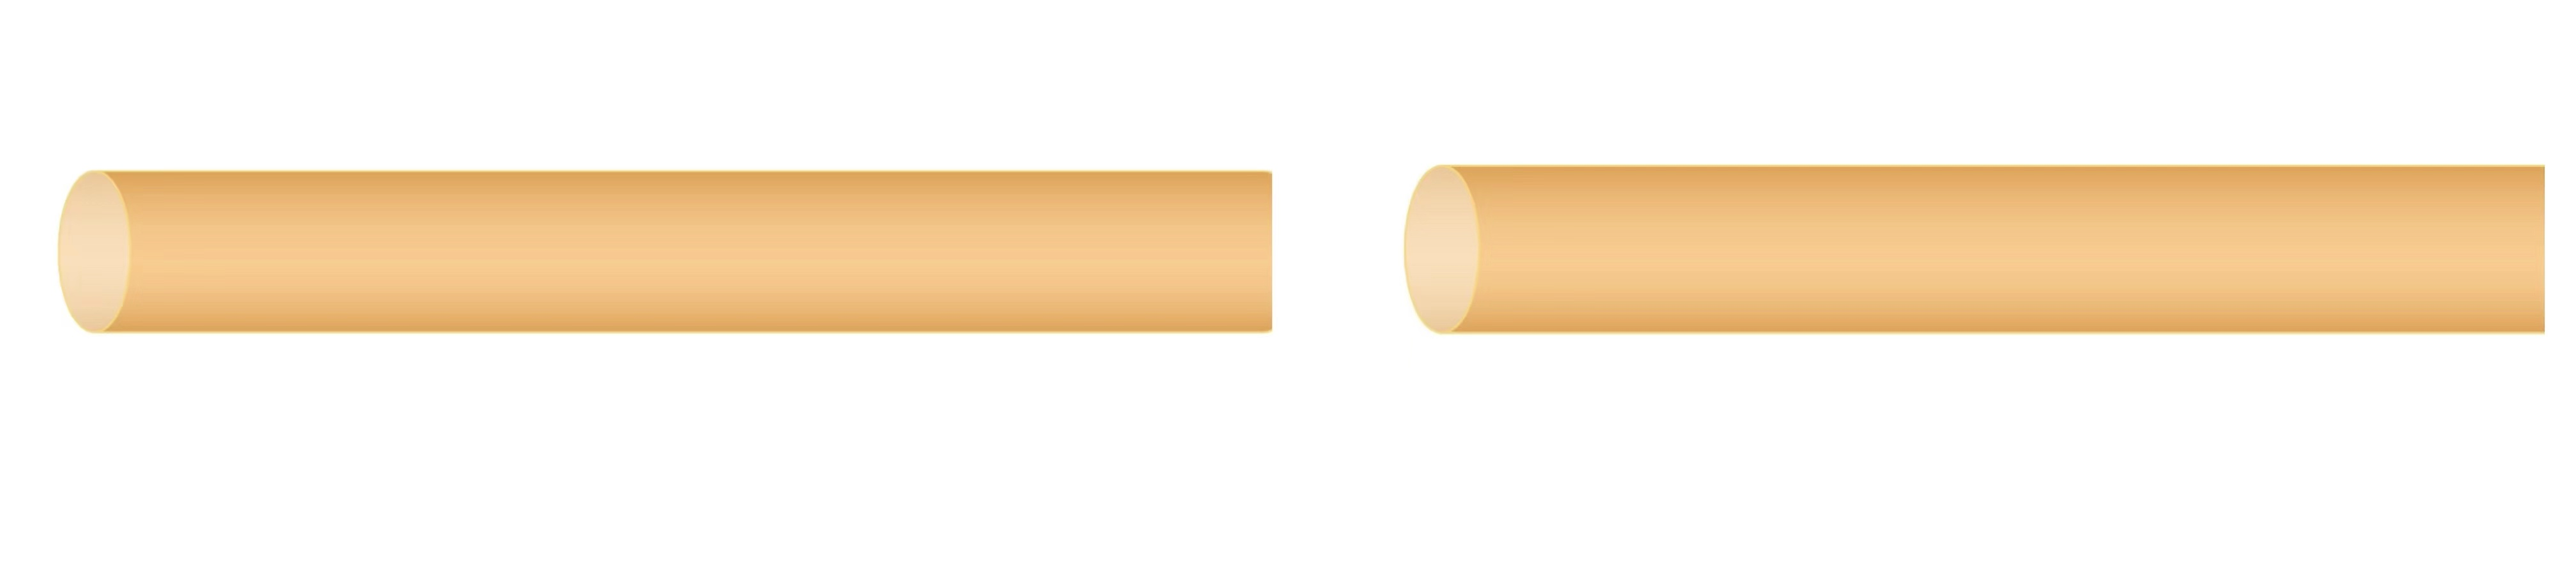
\includegraphics[width=.2\textwidth]{12.jpg}所示,在不叠放的情况下切成五段圆柱需要切几次?(\qquad)
        \begin{tasks}(4)
            \task 1次
            \task 2次
            \task 3次
            \task 4次
        \end{tasks}

        \newpage
        % 13
        \item 观察下列图形规律,虚线框中应该填入的图形是?(\qquad)
        
        \begin{minipage}{.28\textwidth}
            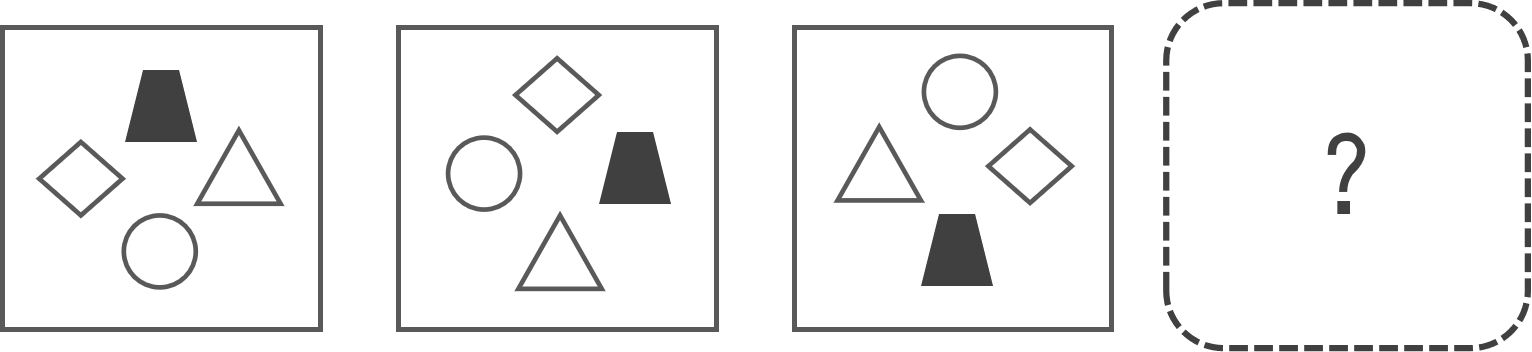
\includegraphics[width=\textwidth]{13.png}
        \end{minipage}
        \begin{minipage}{.65\textwidth}
            \begin{tasks}(4)
                \task 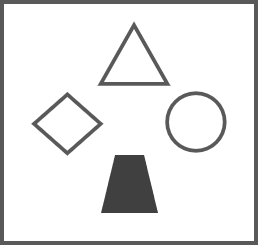
\includegraphics[width=.1\textwidth]{13a.png}
                \task 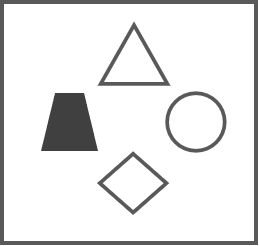
\includegraphics[width=.1\textwidth]{13b.png}
                \task 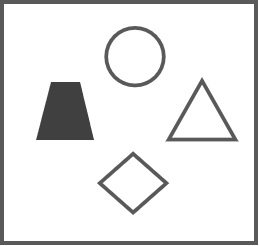
\includegraphics[width=.1\textwidth]{13c.png}
                \task 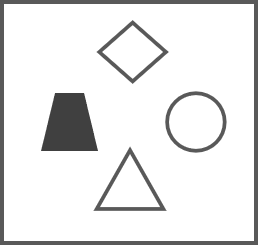
\includegraphics[width=.1\textwidth]{13d.png}
            \end{tasks}
        \end{minipage}
        

        % 14
        \item 两个队伍进行一对一竞赛,队伍一有3个人,队伍二有3个人,要保证每个队员都和对方的三名队员比过一场,应该安排几场比赛?(\qquad)
        \begin{tasks}(4)
            \task 6场
            \task 7场
            \task 8场
            \task 9场
        \end{tasks}

        % 15
        \item 小玉、小林、小明和小红四人在比谁的铅笔多,小玉说:“我的笔比小林多”,小明说:“小红的笔比小林少”,小红说:“小明的笔比我少”,请问四人谁的铅笔最多?(\qquad)
        \begin{tasks}(4)
            \task 小玉
            \task 小林
            \task 小明
            \task 小红
        \end{tasks}

        % 16
        \item 小甲虫的初始状态与位置如下图-左所示。下列选项中,能够让小甲虫爬上下图-右位置并且头朝上的是?(\qquad)
        \begin{tasks}(4)
            \task 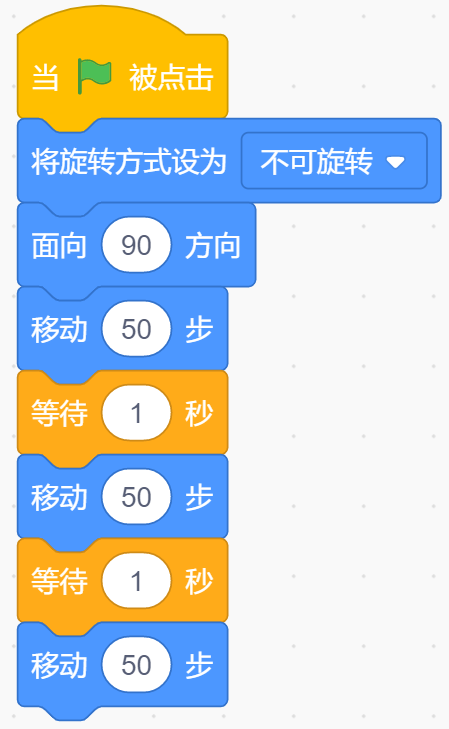
\includegraphics[width=.15\textwidth]{16a.png}
            \task 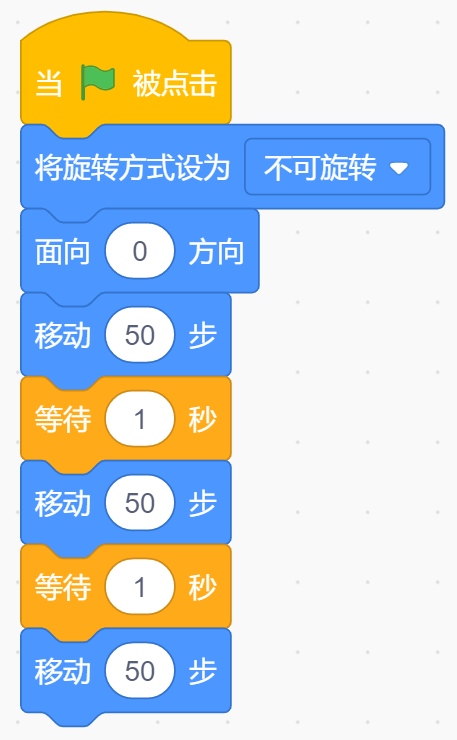
\includegraphics[width=.15\textwidth]{16b.png}
            \task 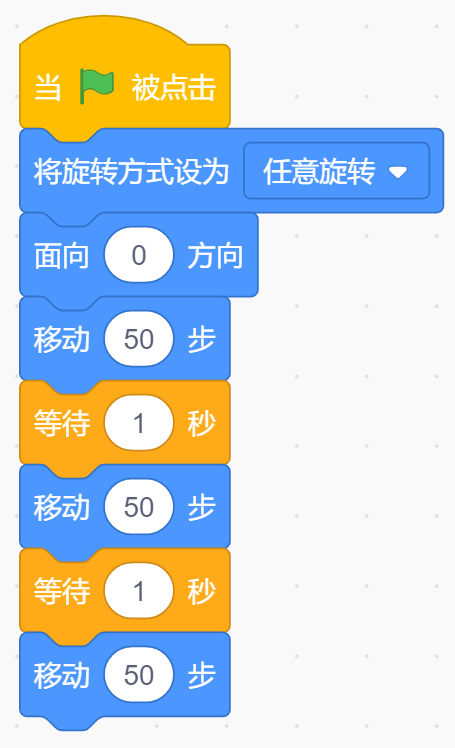
\includegraphics[width=.15\textwidth]{16c.png}
            \task 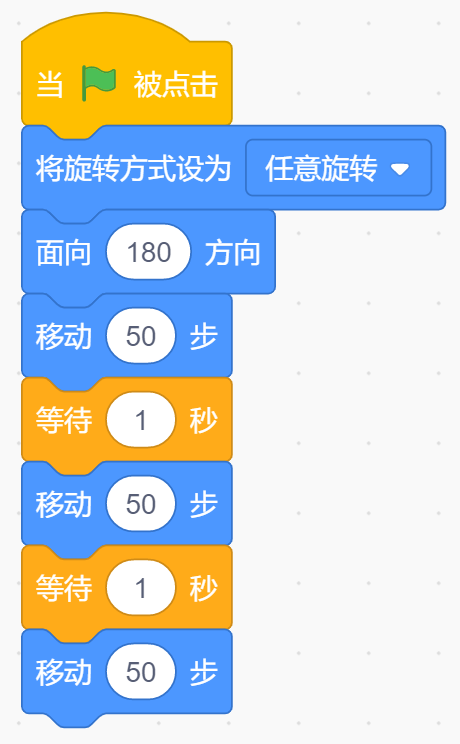
\includegraphics[width=.15\textwidth]{16d.png}
        \end{tasks}

          %     % 13,14,15,16 图片
        \begin{figure}[htbp]
            \centering
            \begin{minipage}[t]{.35\textwidth}
                \centering
                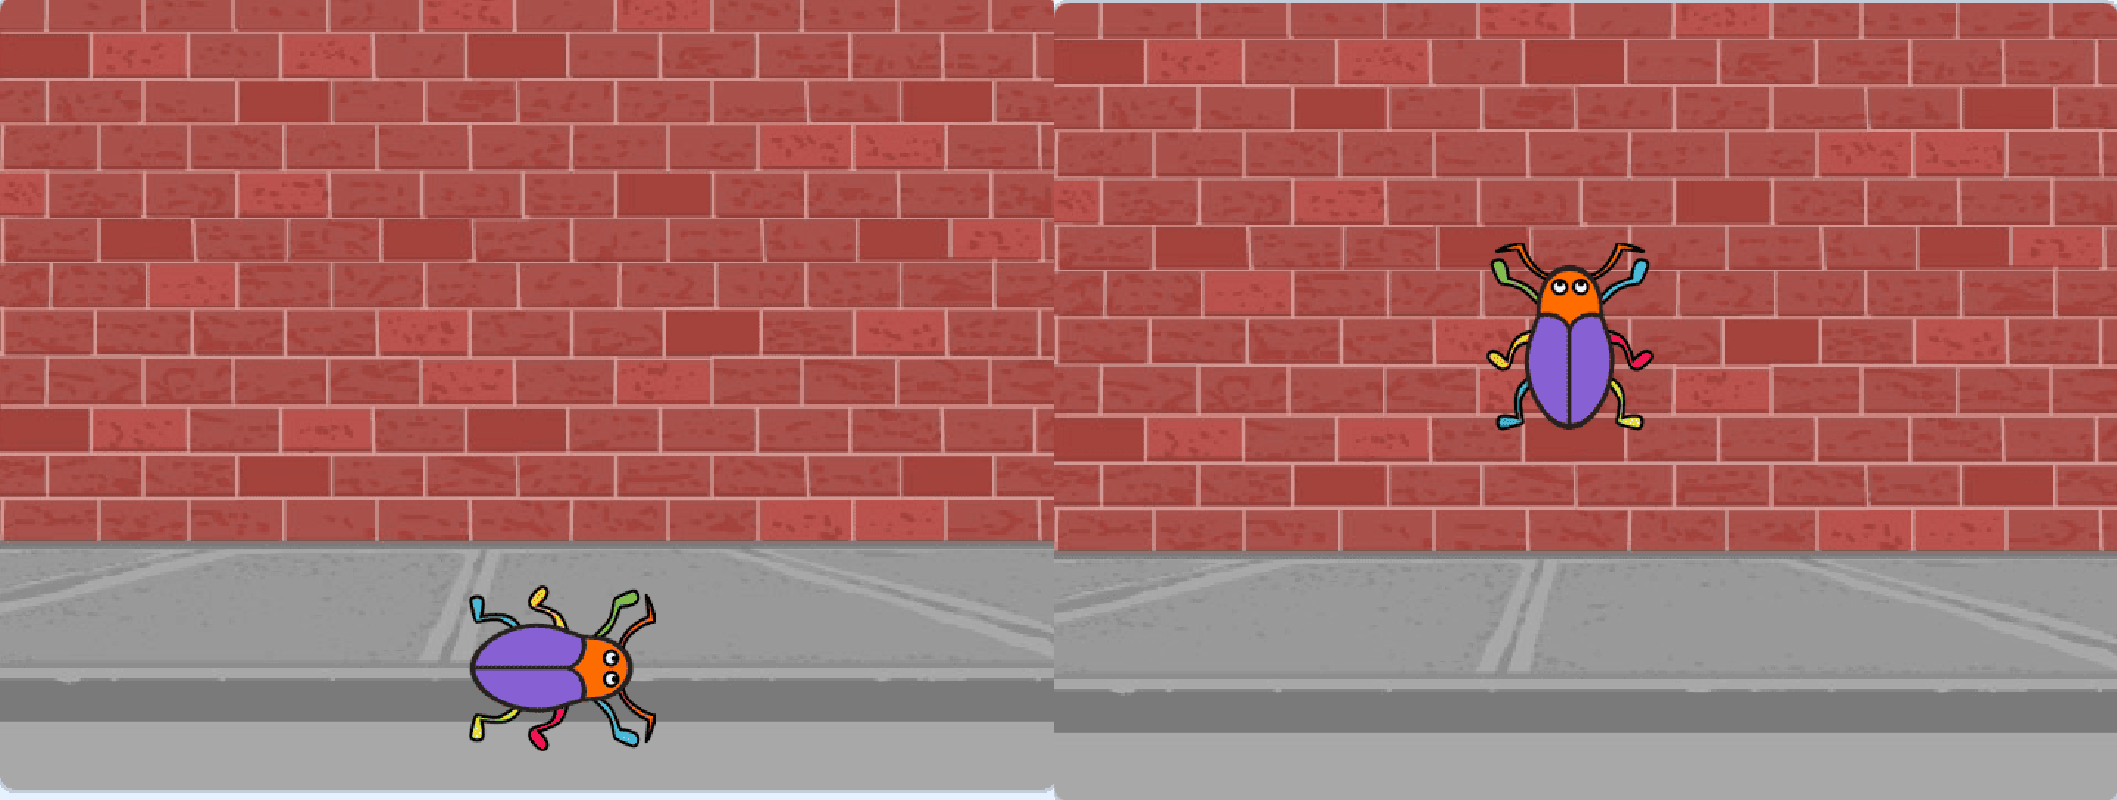
\includegraphics[width=\textwidth]{16.png}
                \caption*{第 16 题}
            \end{minipage}
            \begin{minipage}[t]{.28\textwidth}
                \centering
                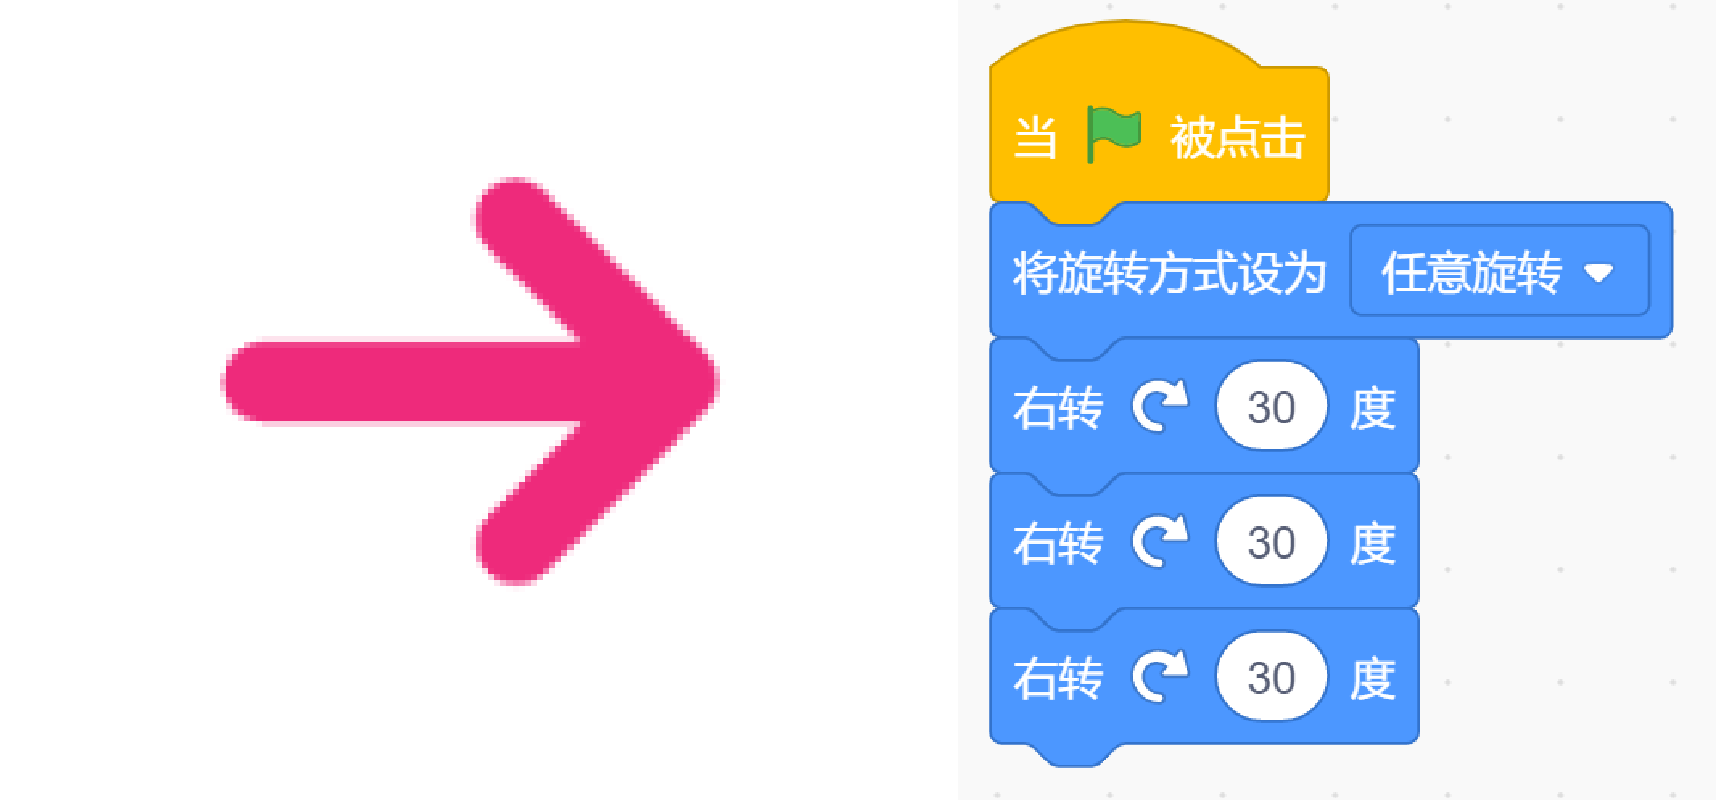
\includegraphics[width=\textwidth]{18.png}
                \caption*{第 18 题}
            \end{minipage}
            \begin{minipage}[t]{.15\textwidth}
                \centering
                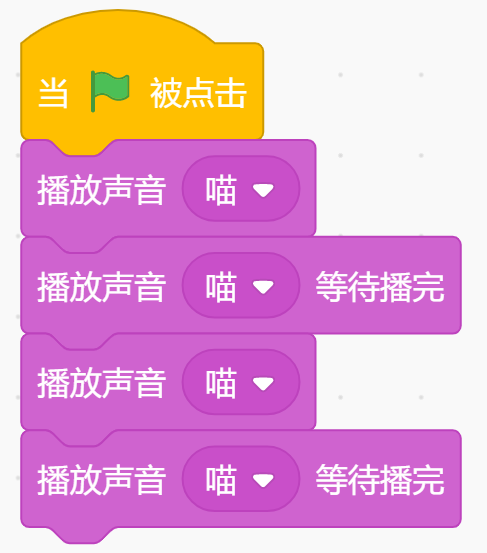
\includegraphics[width=\textwidth]{20.png}
                \caption*{第 20 题}
            \end{minipage}
        \end{figure}

        % 17
        \item 执行下面哪段程序,可以让苹果由
\includegraphics[width=.05\textwidth]{17-1.png}的状态切换到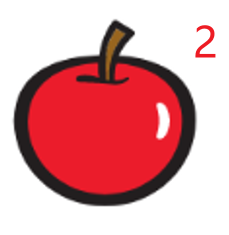
\includegraphics[width=.05\textwidth]{17-2.png}的状态?(\qquad)
        \begin{tasks}(4)
            \task 
\includegraphics[width=.18\textwidth]{17a.png}
            \task \includegraphics[width=.18\textwidth]{17b.png}
            \task \includegraphics[width=.18\textwidth]{17c.png}
            \task \includegraphics[width=.18\textwidth]{17d.png}
        \end{tasks}

        % 18
        \item 角色默认的样式与方向如上图所示,执行程序后,箭头指向的方向为?(\qquad)
        \begin{tasks}(4)
            \task 上
            \task 下
            \task 左
            \task 右
        \end{tasks}

        % 19
        \item 角色的当前音量如图\includegraphics[width=.15\textwidth]{19.png}所示为$70\%$,下面哪个选项能够让声音变小一点?(\qquad)
        \begin{tasks}(4)
            \task \includegraphics[width=.12\textwidth]{19a.png}
            \task \includegraphics[width=.12\textwidth]{19b.png}
            \task \includegraphics[width=.12\textwidth]{19c.png}
            \task \includegraphics[width=.12\textwidth]{19d.png}
        \end{tasks}

        % 20
        \item 执行上图程序,能够听到几声猫叫?(\qquad)
        \begin{tasks}(4)
            \task 1
            \task 2
            \task 3
            \task 4
        \end{tasks}

        \newpage
        % 21
        \item 如下图所示,Ballerina的初始造型为造型3,在\includegraphics[width=.1\textwidth]{21-1.png}积木下需要拼接几块\includegraphics[width=.1\textwidth]{21-2.png}积木,在运行程序后才能让Ballerina换成造型2呢?(\qquad)
        \begin{tasks}(4)
            \task 1块
            \task 2块
            \task 3块
            \task 4块
        \end{tasks}

        % 22
        \item 小猫的初始位置与程序如下图所示,程序执行结束后,小猫停留在哪个区域?(\qquad)
        \begin{tasks}(4)
            \task 1号区域
            \task 2号区域
            \task 3号区域
            \task 4号区域
        \end{tasks}

          % 18,19,20,22,23,24 图片
        \begin{figure}[htbp]
            \centering
            \begin{minipage}[t]{.08\textwidth}
                \centering
                \includegraphics[width=\textwidth]{21.png}
                \caption*{第 21 题}
            \end{minipage}
            \begin{minipage}[t]{.35\textwidth}
                \centering
                \includegraphics[width=\textwidth]{22.png}
                \caption*{第 22 题}
            \end{minipage}
            \begin{minipage}[t]{.45\textwidth}
                \centering
                \includegraphics[width=\textwidth]{23.png}
                \caption*{第 23 题}
            \end{minipage}
            \begin{minipage}[t]{.1\textwidth}
                \centering
                \includegraphics[width=\textwidth]{24-2.png}
                \caption*{第 24 题}
            \end{minipage}
        \end{figure}

        % 23
        \item 舞台上有一个Balloon1角色,Balloon1角色的初始造型和程序如上图所示,点击Balloon1三次后,舞台上显示?(\qquad)
        \begin{tasks}(4)
            \task \includegraphics[width=.08\textwidth]{23a.png}
            \task \includegraphics[width=.06\textwidth]{23b.png}
            \task \includegraphics[width=.1\textwidth]{23c.png}
            \task \includegraphics[width=.1\textwidth]{23d.png}
        \end{tasks}

        % 24
        \item 舞台上有一只小猫如图\includegraphics[width=.2\textwidth]{24-1.png}所示,小猫现在在最左边格子的中心,每走一格需要移动100步,程序如上图所示,要想让小猫走到红色格子的中心,需要点击几次小猫?(\qquad)
            \begin{tasks}(4)
                \task 3次
                \task 4次
                \task 5次
                \task 6次
            \end{tasks}

        % 25
        \item 在哪一个模块下能找到\includegraphics[width=.1\textwidth]{25.png}这块积木?(\qquad)
        \begin{tasks}(4)
            \task \includegraphics[width=.05\textwidth]{25a.png}
            \task \includegraphics[width=.05\textwidth]{25b.png}
            \task \includegraphics[width=.05\textwidth]{25c.png}
            \task \includegraphics[width=.05\textwidth]{25d.png}
        \end{tasks}
    \end{enumerate}

    % 判断题
    \newpage
    {\noindent\textbf{第二部分、判断题(共 10 题,每题 2 分,共20分.)}}
    \begin{enumerate}
        \setcounter{enumi}{25}
        % 26
        \item 只能通过积木块和拖动角色的方式改变角色的坐标。(\qquad)

        % 27
        \item 舞台背景列表如下图所示,想要从背景1切换为Woods背景,使用“下一个背景”积木块和“换成Woods背景”积木块都可以实现。(\qquad)

        % 28
        \item Bear的造型列表如下图所示,使用“下一个造型”积木块,可以让Bear的造型变为bear-a。(\qquad)

        % 29
        \item 母鸡有下列两个造型,执行下列程序后,母鸡的头朝着右边。(\qquad)

        \begin{figure}[htbp]
            \centering
            \begin{minipage}[t]{.08\textwidth}
                \centering
                \includegraphics[width=\textwidth]{27.png}
                \caption*{第 27 题}
            \end{minipage}
            \begin{minipage}[t]{.11\textwidth}
                \centering
                \includegraphics[width=\textwidth]{28.png}
                \caption*{第 28 题}
            \end{minipage}
            \begin{minipage}[t]{.3\textwidth}
                \centering
                \includegraphics[width=\textwidth]{29.png}
                \caption*{第 29 题}
            \end{minipage}
            \begin{minipage}[t]{.3\textwidth}
                \centering
                \includegraphics[width=\textwidth]{32.png}
                \caption*{第 32 题}
            \end{minipage}
            \begin{minipage}[t]{.18\textwidth}
                \centering
                \includegraphics[width=\textwidth]{33.png}
                \caption*{第 33 题}
            \end{minipage}
        \end{figure}

        % 30
        \item 每上一层楼需要走10阶楼梯,李华从1楼走到4楼一共走了40阶楼梯。(\qquad)

        % 31
        \item 对于默认的小猫角色,将旋转方式设为不可旋转,小猫面向 $-90$,小猫会倒立。(\qquad)

        % 32
        \item 角色1的面向方向与旋转方式可以编程用积木修改,也可以在如上图所示的区域修改。(\qquad)

        % 33
        \item 小鸡的造型列表与程序如上图所示,运行程序后,可以清楚地看见小鸡一边向左移动一边切换造型。(\qquad)
        
        % 34
        \item 在背景中用\includegraphics[width=.15\textwidth]{34.png}积木块调整音量,角色中的声音音量也会跟着变化。(\qquad)

        % 35
        \item Scratch中只能给角色添加一个声音。(\qquad)
    \end{enumerate}

    \newpage
    {\noindent \textbf{第三部分、编程题(共 2 题,共30分.)}}
    \begin{enumerate}
        \setcounter{enumi}{35}
        
        % 36
        \item 旅行相册:
        
        1. 准备工作
        \begin{tasks}[label = (\arabic*)]
            \task 删除小猫角色;
            \task 选择角色Wizard-toad;
            \task 删除默认白色背景,选择背景依次为:Forest, Boardwalk, Water And Rocks, Arctic;
            \task 给背景选择声音Chill。
        \end{tasks}
        2. 功能实现
        \begin{tasks}[label = (\arabic*)]
            \task 点击绿旗开始,角色Wizard-toad初始位置如图所示,初始造型为wizard-toad-a;
            \task 程序开始1秒后,角色Wizard-toad向上跳起100步,换成wizard-toad-b造型,在空中停留1秒后,落到地面,换成wizard-toad-a造型,注意角色
            Wizard-toad始终朝向右;
            \task 点击绿旗后,初始背景为Forest,背景播放着声音Chill,同时每隔1秒切换一次背景,最后停在第四个背景Arctic。
        \end{tasks}
        \begin{figure}[htbp]
            \centering
            \includegraphics[width=.26\textwidth]{36.png}
        \end{figure}

        %37
        \item 报时公鸡:
        
        1. 准备工作
        \begin{tasks}[label = (\arabic*)]
            \task 背景:根据下图绘制两张背景;
            \task 删除默认角色,添加角色Rooster\includegraphics[width=.05\textwidth]{37-2.png}。
        \end{tasks}
        2. 功能实现
        \begin{tasks}[label = (\arabic*)]
            \task 点击绿旗,角色Rooster初始化位置、大小,位于舞台左侧,面向右侧,造型为“rooster-a”,背景为“背景1”;
            \task 点击角色Rooster,Rooster从舞台左侧走到右侧,再从右侧走到中间;(注意走的过程中脚不能朝上,并且朝哪个方向走Rooster就面朝哪里);
            \task 走完后,切换成造型“rooster-b”,播放声音"rooster",声音播完后,切换背景为“背景2"。
        \end{tasks}

        \begin{figure}[htb]
            \centering
            \begin{minipage}[t]{.24\textwidth}
                \centering
                \includegraphics[width=.9\textwidth]{37-1.png}
            \end{minipage}
            \begin{minipage}[t]{.24\textwidth}
                \centering
                \includegraphics[width=.9\textwidth]{37-3.png}
            \end{minipage}
            \begin{minipage}[t]{.24\textwidth}
                \centering
                \includegraphics[width=.9\textwidth]{37-4.png}
            \end{minipage}
            \begin{minipage}[t]{.24\textwidth}
                \centering
                \includegraphics[width=.9\textwidth]{37-5.png}
            \end{minipage}
        \end{figure}
    \end{enumerate}
\end{document}